\documentclass[12pt]{article}

\usepackage{color}
\usepackage{amsmath,amssymb}
\usepackage{graphicx}
\usepackage{listings}

\title{Interpreting the Correlation between Temperature and Year using TAutoCorr.R}
\author{Talia Al-Mushadani}
\date{}

\begin{document}
    \maketitle

    \section{Examining the Key West data}
    Firstly, I set about examining the variables and the class of these variables 
    listed in the Key West Annual Mean Temperature data by using str.
    I then plotted the data that we were provided with to discover what the 
    basic shape of the data looked like, which is shown in figure 1. 
    I found that there were two variables included, year and temperature, 
    and that temperature seemed to increase as time, in years, went on.
    
    \begin{figure}
        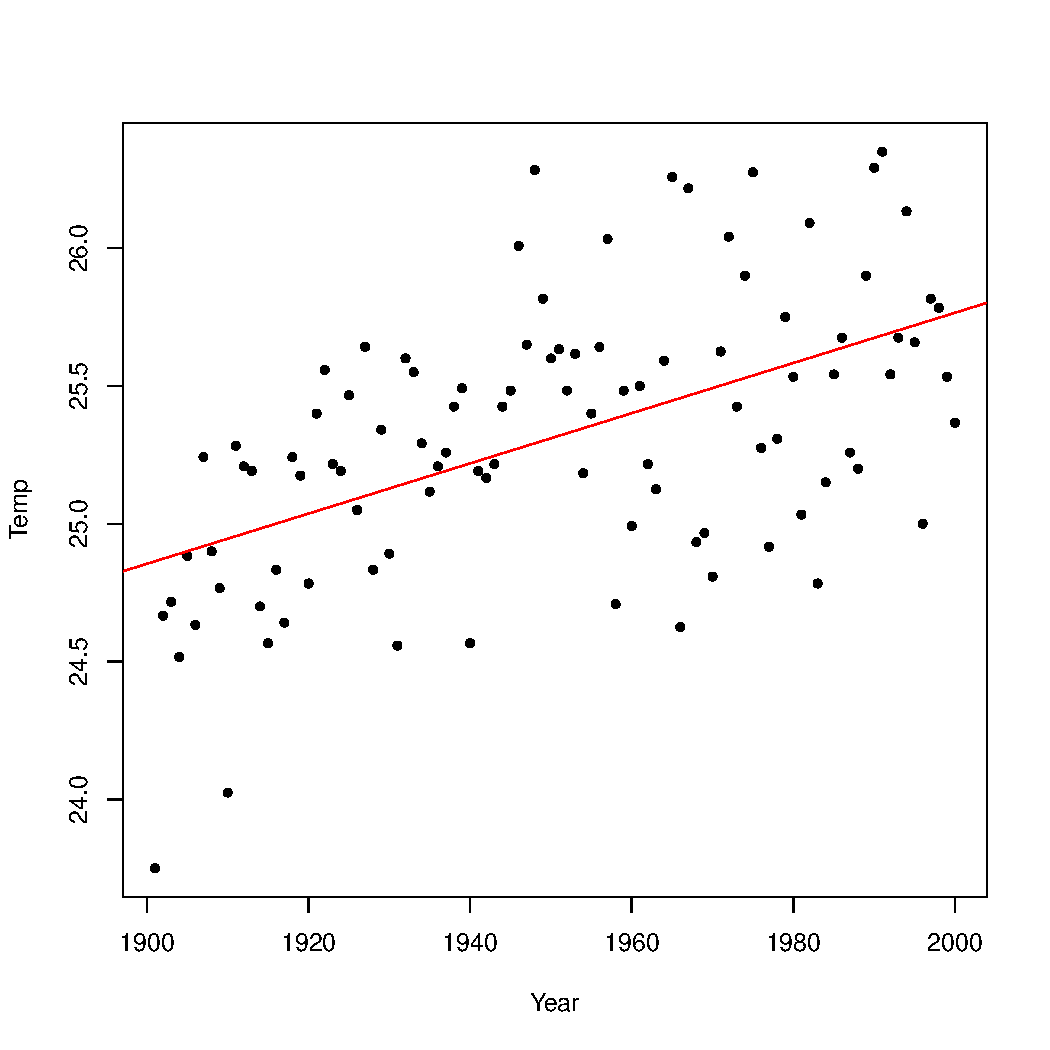
\includegraphics[width = 1\textwidth]{KeyWestScatter.pdf}
        \caption{Figure 1. A graph displaying the variation in temperature 
        over the years in the Key West data and a linear model attempting to displaying
        what the relationship between the temperature and years may be.}
    \end{figure}

    \section{Assessing the possible correlation between temperature in successive years}
    I, initially, calculated what the correlation between successive years' temperature
    in the correct time series order, finding that the coefficient is equal to 0.33,
    with the correlation calculated by comparing the difference in temperature between
    n - 1 pairs of years, when n is the number of years.
    I, then, randomly sampled the temperature so that the time series becomes jumbled,
    and any correlation that does occur between successive years' temperature would be
    disrupted. This process was repeated 10000, and the correlation between the
    temperatures in each permuation of the time series was calculated.
    To see what the distribution of the random correlation coefficients, I plotted a
    histogram and then included a line indicating the correlation coefficient of
    the correct time series data, to allow me to compare them, as shown in figure 2 below. 
    I then calculated the approximate p value, by dividing the number of
    permutations that gave a correlation greater than TempCor by the number of
    permutations, which I found to be equal to 0.0004.

    \begin{figure}
        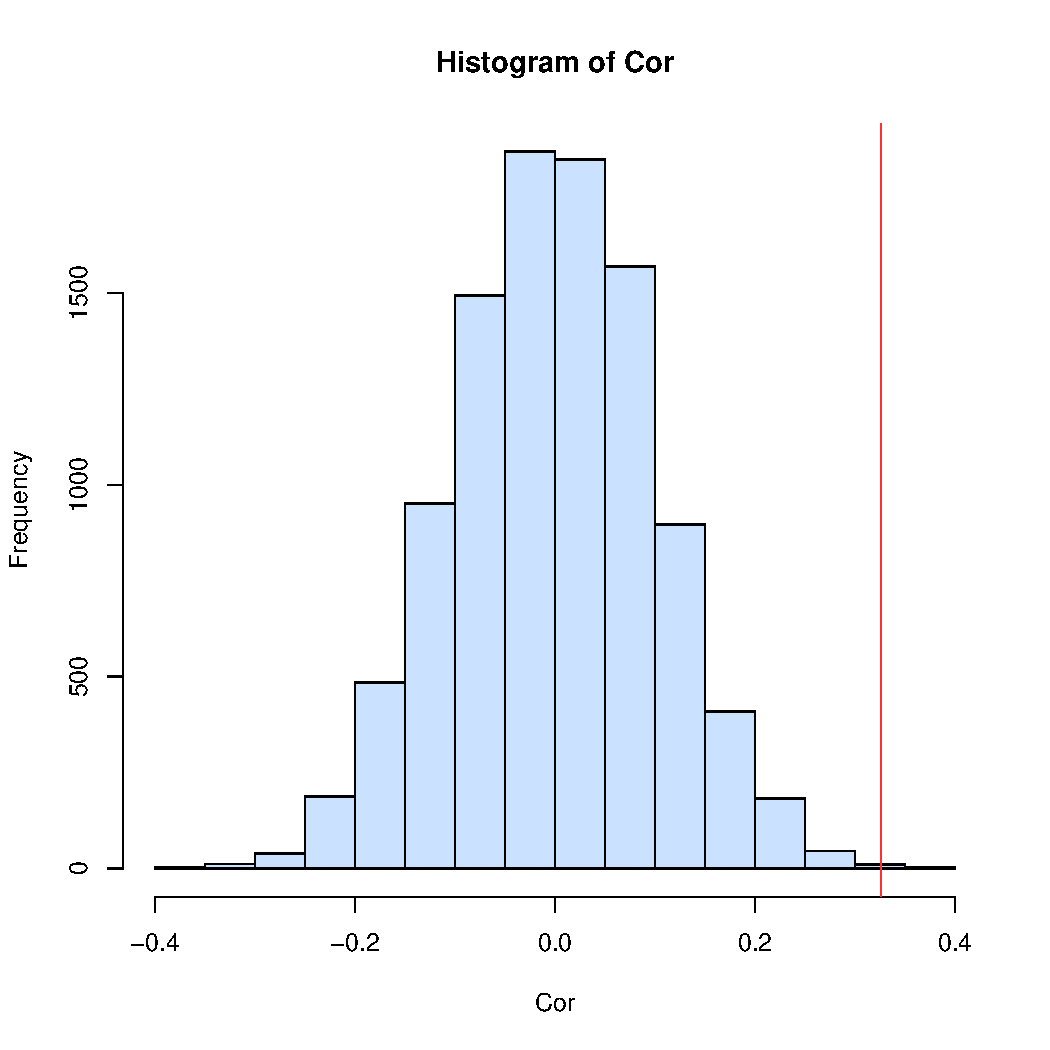
\includegraphics[width = 1\textwidth]{TAutoCorr_histogram.pdf}
        \caption{Figure 2. A graph displaying the distribution of the sampled time series
        correlations and its' relation to the correlation of the correctly ordered time
        series.}
    \end{figure}
    

    \section{Interpreting our results}
    The randomly sampled time series act as a data set from which the null hypothesis
    for a correlation between the successive years can be produced. By comparing the
    chances of randomly achieving the correlation coefficient with the correlation
    coefficient achieved with the correct time series, we are able to see that whilst
    there is a proportion of scrambled time series that gave greater correlations than
    the original, that proportion is so small that it could be considered insignificant.
    This is highlighted by the fact that the standard p-value or proportion used to 
    determine whether we can reject the null hypothesis, is only 0.05, which is 125 times
    greater in size than the approximate p-value I calculated. As such we are able to
    reject the null hypothesis, that there is no statistical significance to the
    correlation initially determined, despite the seemingly low value of the correlation.

\end{document}